\documentclass{article}

\usepackage{graphicx}
\usepackage[hidelinks]{hyperref}
\usepackage[a4paper, total={6in, 8in}]{geometry}
\usepackage[slovak]{babel}
\usepackage{caption}
\usepackage{subcaption}

\graphicspath{./include/}

\renewcommand{\figurename}{Obr.}
\renewcommand{\contentsname}{Obsah}

\begin{document}

\begin{titlepage}
	\null\vfill

	\begin{center}
		{\Huge Meranie a aproximácia prevodovej charakteristiky tepelného systému }
		\vskip 2cm

		{\Large Cvičenie č. 11}
		\vskip 0.5cm

		{\large Spojité procesy}
	\end{center}

	\vfill
	\vfill

	\begin{flushright}
		Filip Lobpreis \\
		Matúš Machata \\
		\small\today\\
	\end{flushright}
	\hfill
\end{titlepage}

\thispagestyle{empty}
\clearpage

\tableofcontents
\thispagestyle{empty}
\clearpage

\section{Zadanie}
\label{sec:zadanie}
\pagenumbering{arabic}

\begin{figure}[!htbp]
	\begin{center}
		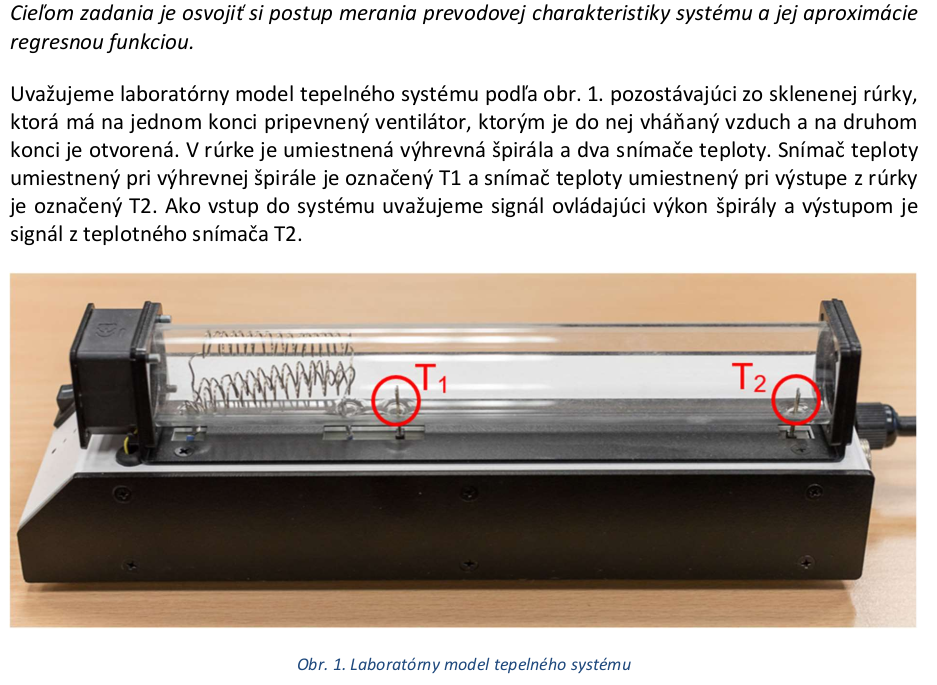
\includegraphics[width=0.8\textwidth]{./include/zadanie.png}
	\end{center}
	\caption{Prvá časť zadania z~cvičenia č. 11 z~predmetu spojité procesy}
	\label{fig:zadanie1}
\end{figure}

\clearpage

\section{Teória}
\label{sec:teoria}

V~tomto zadaní je našou úlohou experimentálne overiť návrh regulácie výšky hladiny na~laboratórnom
modeli tepelného systému a~overiť navrhované riešenie. Pri~tomto zadaní sme použili už~preddefinovanú schému
v~programe \textit{Simulink} (Obr.~\ref{fig:schema}).

\begin{figure}[!htbp]
	\begin{center}
		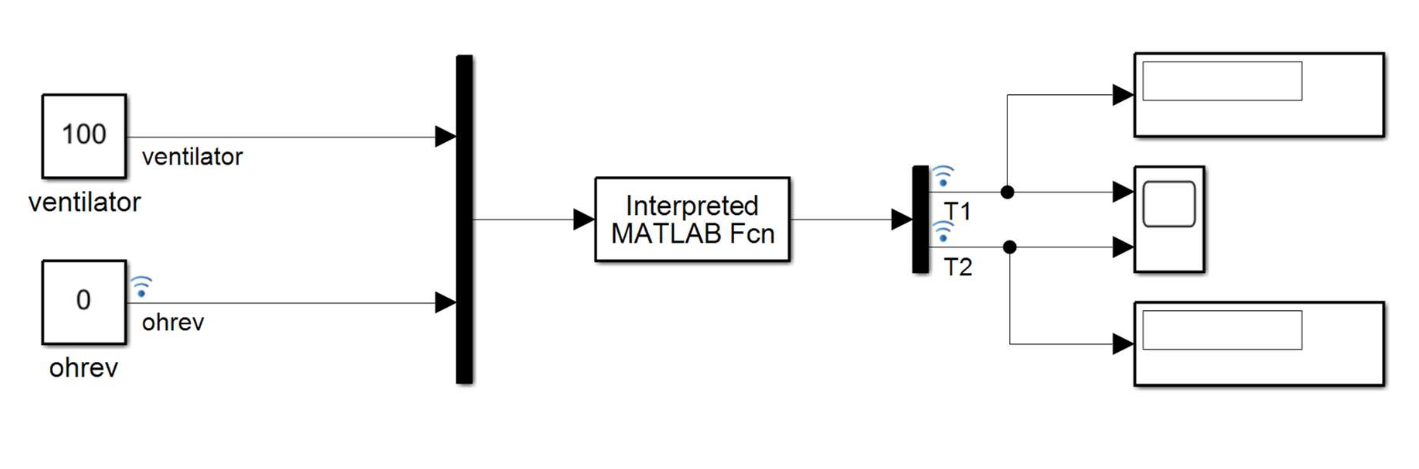
\includegraphics[width=0.8\textwidth]{./include/schema.png}
	\end{center}
	\caption{Schéma modelu z~cvičenia č. 11 z~predmetu spojité procesy}
	\label{fig:schema}
\end{figure}

V~tomto zapojení vidíme viacero vstupných signálov, tie sú už~preddefinované. \textbf{ventilator} reprezentuje
na koľko percent funguje ventilátor v systéme. \textbf{ohrev} reprezentuje vstupný signál ohrevnej špirály,
jeho hodnoty sú zadávané v~percentách. Túto hodnotu budeme v priebehu merania prestavovať. Bude sa meniť
od 0\% po 100\% s krokom 10\%.

\clearpage

\subsection{Úvod do~priebehu simulácie}
\label{subsec:priebehSimulacie}

Na~obrázku Obr.~\ref{fig:mt2} je znázornený priebeh simulácie tepelného systému s ohrevnou špirálou. Na začiatku
merania sme nastavili ohrev špirály na 10\%. Postupne sme zvyšovali hodnotu ohrevu až k~100\%. Keďže sme prvú
hodnotu nenastavili na 0\%, tak sme meranie zopakovali. Pri druhom meraní sme dostali hodnoty, ktoré boli vyššie
ako hodnoty z prvého merania. Pri aproximácia budeme použivať hodnoty z druhej časti merania.

\begin{figure}[!htbp]
	\begin{center}
		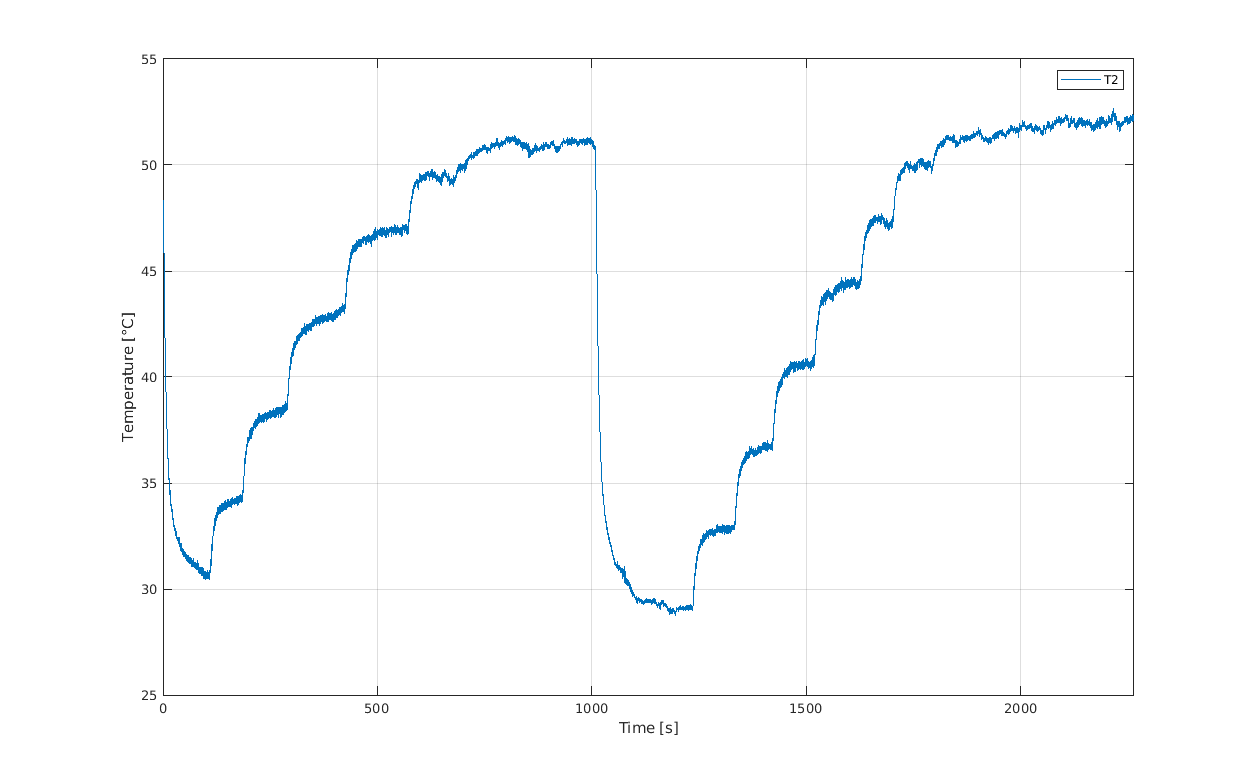
\includegraphics[width=\textwidth]{./include/teplota_2.png}
		\caption{Priebeh meranej teploty na snímači T2.}
		\label{fig:mt2}
	\end{center}
	\hfill
\end{figure}

Merané hodnoty z druhej časti nám vyšli následovne:

\begin{center}
\begin{tabular}{ |c|c|c| }
 \hline
 ohrev [\%] & T1 [$^\circ $C] & T2 [$^\circ $C] \\
 \hline
   0 & 29.3 & 29 \\
  10 & 33.5 & 33 \\
  20 & 38 & 37 \\
  30 & 42 & 41\\
  40 & 46.5 & 45\\
  50 & 49.5 & 47.5\\
  60 & 52.5 & 50 \\
  70 & 54 & 51.3 \\
  80 & 54.5 & 51.6 \\
  90 & 55 & 52 \\
 100 & 55 & 52 \\
 \hline
\end{tabular}
\end{center}
\newpage

\section{Lineárna aproximácia}
\label{sec:lin}

\begin{figure}[!htbp]
	\begin{center}
		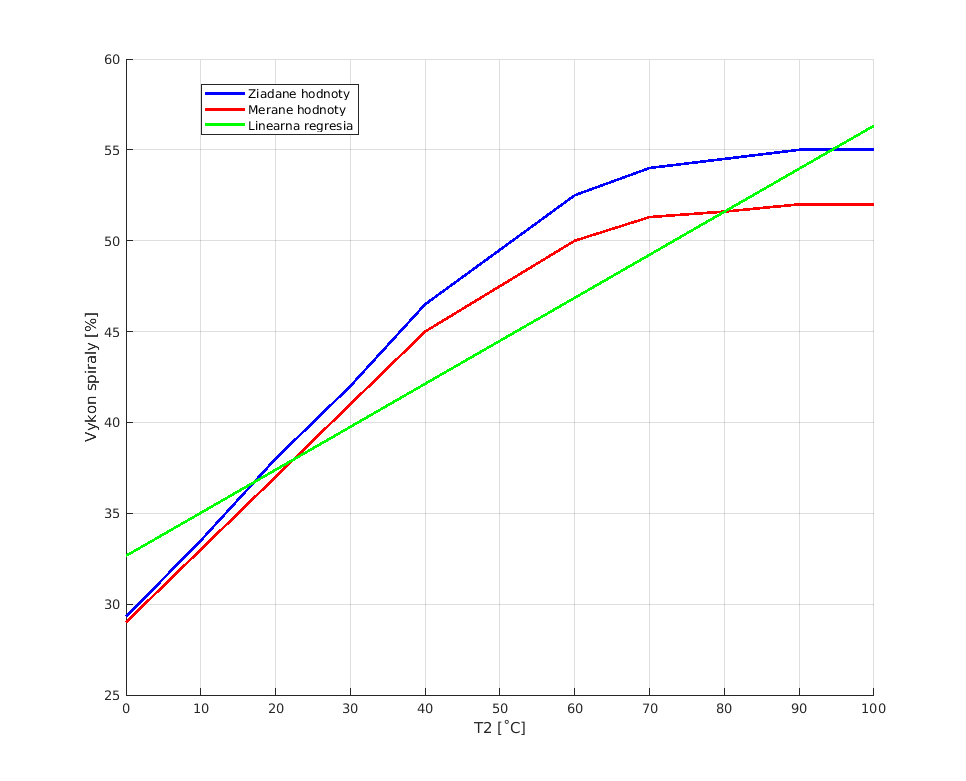
\includegraphics[width=\textwidth]{include/linearna_regresia.png}
	\end{center}
	\caption{Lineárna aproximácia tepelného systému.}
	\label{fig:linApx}
\end{figure}

Odhadnutý funkčný vzťah:

\begin{equation}
	\hat{y} = \hat{\theta}_0 + \hat{\theta}_1u
	\label{eq:linApx}
\end{equation}

Vztah \ref{eq:linApx} mozeme prepisat do maticoveho tvaru:
\begin{equation}
	\hat{y} = H_1\hat{\theta}_1
	\label{eq:linApx2}
\end{equation}

kde tieto moatice mozeme vyjadrit nasledovne:

\begin{figure}[!htbp]
	\begin{center}
		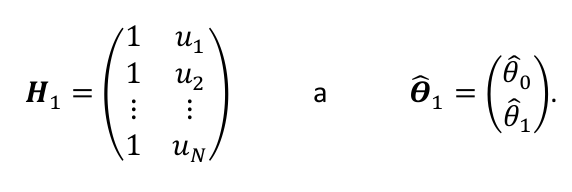
\includegraphics[width=0.25\textwidth]{include/defHandTheta.png}
	\end{center}
\end{figure}

Lineárna aproximácia je najjednoduchšia aproximácia, ktorá sa používa pri aproximácii prevodovej
charakteristiky. Na jej prevedenie sme vytvorili maticu \textbf{H}, vypočítali
\(\theta\) Gaussovým vzťahom
\begin{equation}
	\theta = (H^TH)^{-1}H^Ty
	\label{eq:gausEq}
\end{equation}

a následne sme pomocou vzťahu \(y_1 = H_1\theta_1\) vyjadrili funkciu opisujúcu funkciu pre výstupné
veličiny.

Hodnoty účelovej funkcie sme si vypočítali zo vzťahu 
\begin{equation}
	Q1 = \frac{1}{2} e^Te
	\label{eq:objFunkcia}
\end{equation}

Obr.~\ref{fig:linApx} ukazuje priebeh linearnej aproximácie tepelneho systemu a
Obr.~\ref{fig:prevod} zobrazuje porovnanie prevodových funkcií s lineárnou aproximáciou.


\clearpage

\section{Kvadraticka aproximacia}
\label{sec:kvad}

\clearpage

\section{Odmocninova aproximacia}
\label{sec:odm}

\clearpage



\section{Zhrnutie}
\label{sec:zhrnutie}

\begin{figure}[!htbp]
	\begin{center}
		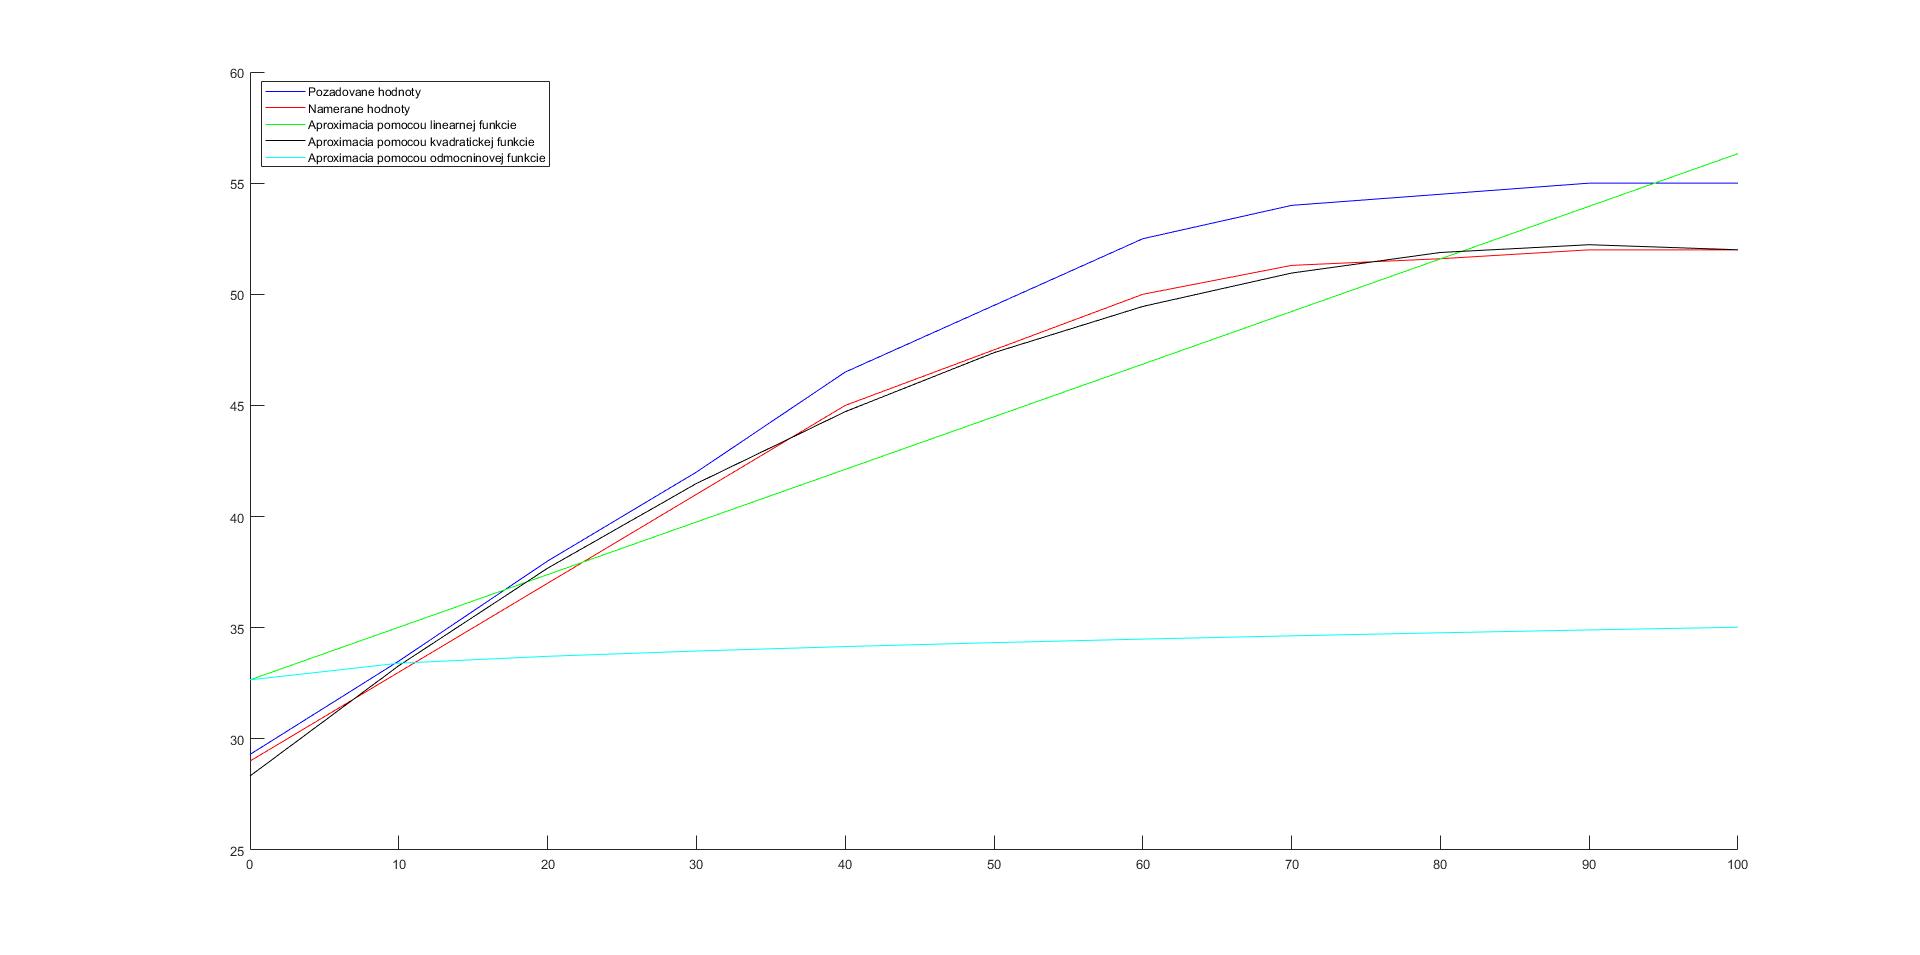
\includegraphics[width=\textwidth]{./include/prevodove_funkcie.png}
		\caption{Priebeh prevodových funkcii}
		\label{fig:prevod}
	\end{center}
	\hfill
\end{figure}


\end{document}

